% Group report, IEEE conference format. The divide-and-conquer half lives in
% divide_and_conquer/sec_dc.tex / app_dc.tex, the greedy half in
% greedy/sec_greedy.tex / app_greedy.tex. Work still owed would be marked with the red
% placeholder macro below; none remains.
%
% To build on Overleaf: upload the whole repository, keep the file layout, compile with
% pdfLaTeX. Nothing needs installing.
\documentclass[conference]{IEEEtran}
\IEEEoverridecommandlockouts
\usepackage{cite}
\usepackage{amsmath,amssymb,amsfonts}
\usepackage{amsthm}
\usepackage{algorithmic}
\usepackage{graphicx}
\usepackage{textcomp}
\usepackage{xcolor}
\usepackage{url}
\usepackage{listings}

% Theorem-like environments with air around them. IEEEtran's defaults have
% no vertical space, which makes a run of lemmas and proofs hard to read.
\newtheoremstyle{spaced}
  {10pt plus 2pt minus 2pt}  % space above
  {10pt plus 2pt minus 2pt}  % space below
  {\itshape}                 % body font
  {}                         % indent
  {\itshape}                 % head font
  {:}                        % punctuation after head
  {.5em}                     % space after head
  {}                         % head spec (default)
\theoremstyle{spaced}
\newtheorem{lemma}{Lemma}
\newtheorem{theorem}{Theorem}
\newtheorem{corollary}{Corollary}
\renewenvironment{IEEEproof}[1][\IEEEproofname]{\par\vspace{4pt}%
  \noindent\hspace{\parindent}{\itshape #1: }\ignorespaces}%
  {\hfill\IEEEQED\par\vspace{6pt}}

% Code listings (Appendix A) and the Lean proof (Appendix B).
\lstset{basicstyle=\ttfamily\scriptsize, breaklines=true, columns=fullflexible,
  frame=single, keepspaces=true, showstringspaces=false,
  % Unicode symbols in the Lean listing, mapped to math symbols.
  literate={≤}{{$\le$}}1 {≠}{{$\ne$}}1 {∧}{{$\wedge$}}1 {∨}{{$\vee$}}1
           {¬}{{$\neg$}}1 {↔}{{$\leftrightarrow$}}1 {→}{{$\rightarrow$}}1
           {∀}{{$\forall$}}1 {∃}{{$\exists$}}1 {⟨}{{$\langle$}}1 {⟩}{{$\rangle$}}1
           {×}{{$\times$}}1 {α}{{$\alpha$}}1 {∈}{{$\in$}}1 {·}{{$\cdot$}}1
           {₁}{{$_1$}}1 {₂}{{$_2$}}1 {⊢}{{$\vdash$}}1
           {⌈}{{$\lceil$}}1 {⌉}{{$\rceil$}}1 {⌊}{{$\lfloor$}}1 {⌋}{{$\rfloor$}}1}

% Work still owed by the greedy half, printed in red so nothing is missed.
\newcommand{\partnertodo}[1]{\textcolor{red}{\textbf{[Partner: #1]}}}

% Folder holding the divide-and-conquer figures and code.
\newcommand{\dcdir}{divide_and_conquer/}

\begin{document}

\title{Greedy and Divide-and-Conquer Algorithms for Real-World Problems}

\author{\IEEEauthorblockN{Ilan Danial}
\IEEEauthorblockA{\textit{Dept.\ of Computer \& Information Science \& Engineering} \\
\textit{University of Florida}\\
Gainesville, FL, USA \\
ilan.danial@ufl.edu}
\and
\IEEEauthorblockN{Ryan Rodriguez}
\IEEEauthorblockA{\textit{Dept.\ of Computer \& Information Science \& Engineering} \\
\textit{University of Florida}\\
Gainesville, FL, USA \\
rrodriguez7@ufl.edu}
}

\maketitle

\begin{abstract}
A cruise-fare tracker that reads an unofficial, rate-limited search API
should call it as rarely as it can. We model quote requests with acceptable
date windows as integer intervals and choose the fewest refresh days that hit
every window, a minimum point cover that a greedy scan by closing day solves
optimally in $O(n\log n)$ time; on $383$ real Carnival sailings it needs three
refreshes.
Map-search sites cap the number of listings shown per window, so collecting
every listing in a city means choosing windows that never overflow. We model
this as a point set on an integer grid and give a divide-and-conquer algorithm
that recursively splits overflowing windows into quadrants. We prove it
correct and bound its recursion depth by $\lceil\log_2 W\rceil$ for a map of
$W$ grid units; every statement is machine-checked in Lean~4. For evenly
spread listings it makes $\Theta(n/k)$ requests and $\Theta(n\log(n/k))$
work, which experiments confirm on synthetic data and on 261 real Airbnb
listings.
\end{abstract}

\begin{IEEEkeywords}
greedy algorithm, interval point cover, web scraping, rate limiting, cruise
fares, divide and conquer, quadtree,
formal verification
\end{IEEEkeywords}

\section{Introduction}

This report applies two algorithm-design techniques to problems that arose
outside the classroom. For each we state the problem, abstract it, give an
algorithm with a running-time analysis and a proof of correctness, explain the
algorithm in the problem's own terms, and check the analysis experimentally.

Both problems come from scraping travel marketplaces under a limit the
platform imposes. The divide-and-conquer half asks \emph{where} to look when a
map caps the results per window; the greedy half asks \emph{when} to look
when an API caps how often one may ask. Section~\ref{sec:greedy} takes a
cruise-fare tracker that reads Carnival's unofficial, rate-limited search
endpoint. We propose letting users ask for one fresh quote per sailing within
a window of days, and choose the fewest refresh batches that serve every
window. This is the minimum point cover of intervals. A greedy scan by
closing day is optimal, which we prove with a set of pairwise disjoint
witness windows, and runs in $O(n\log n)$ time, which experiments confirm up
to $n=2^{22}$. On $383$ real sailings it needs three refreshes over six
months.

The second problem comes from web data collection. A map-search service
shows at most $k$ listings for any map window, so a scraper that needs every
listing in a city must split the map into windows that never overflow, using
as few requests as it can. Section~\ref{sec:dc} models the map as an integer
grid and the service as a capped oracle, solves the problem with a
divide-and-conquer recursion on quadrants, proves the recursion correct and
bounds its depth by $\lceil\log_2 W\rceil$, and verifies the predicted
$\Theta(n\log(n/k))$ cost experimentally. Every statement in the correctness
section is also machine-checked in Lean~4 (Appendix~\ref{app:dc-lean}).

% Greedy half of the report. Uses the same preamble as sec_dc.tex.
% Figures are read from greedy/ because report.tex lives in the repository root.

\section{Greedy: Fewest Price Refreshes Under a Request Budget}
\label{sec:greedy}

\subsection{Problem}
\label{sec:greedy-problem}

Fare trackers learn of price changes only by querying the seller's site, as
in early airfare-prediction work~\cite{etzioni2003buy}, and a site may refuse
requests that arrive too fast~\cite{rfc6585}.
Cruise Finder~\cite{cruisefinder} is a self-hosted web application, written
by the second author, that tracks Carnival Cruise Line sailings from Florida.
It reads prices from Carnival's public but undocumented search endpoint,
calling it once per configured departure month and following every result
page. Because the endpoint is unofficial and rate-limited, the application
calls it only on demand and logs every call in an append-only audit table.
We call one pass over every configured month and every page a \emph{refresh
batch}; it observes the current price of every listed sailing. We assume
every batch costs the same, so the objective counts batches, not HTTP
requests (the number of pages can change over time).

We propose a feature that the application does not have today: \emph{quote
requests}. A quote request names a sailing and a window of days during which
one fresh observation of its price is acceptable. The question is: given every
request's window, what is the fewest refresh batches that give every window at
least one observation, and on which days?

For the case study we generate one request per sailing by a stated policy, a
modeling choice rather than a claim about how fares move. Each window opens at
Carnival's final-payment deadline, $76$ days before departure for cruises of
up to $5$ days and $91$ days for $6$ days or more~\cite{carnival481}, and
closes when booking closes, $c$ days before departure. Final payment is when
every booking must be paid in full; unpaid bookings are cancelled and their
cabins return to sale, so it is a natural moment to want a current quote. We
found no Carnival page giving the booking cutoff, so $c=2$ is an assumption.
The model asks for one observation per window, not continuous tracking, so it
minimizes refresh batches, not missed discounts or the average staleness that
crawler refresh policies optimize~\cite{cho2003refresh}.

\subsection{Abstraction}
\label{sec:greedy-abstraction}

Days are integers. Sailing $i$ departs on day $d_i$ and lasts $L_i$ days;
its window is $W_i=[a_i,b_i]$ with
\begin{equation}
a_i=d_i-F(L_i),\quad b_i=d_i-c,\quad
F(L)=\begin{cases}76 & L\le5,\\ 91 & L\ge6.\end{cases}
\label{eq:greedy-window}
\end{equation}
We take $L_i$ from the search data's duration field, which equals arrival
minus departure in days for every sailing we fetched and matches the
``$L$-Day'' length the table in~\cite{carnival481} uses. Windows with $b_i$ before
today are dropped, and $a_i$ is raised to today if it is earlier. A batch on
day $t$ observes every window with $t\in W_i$.

The abstract problem: given a set $\mathcal{W}=\{W_1,\dots,W_n\}$ of integer
intervals with $a_i\le b_i$, find a set of days $T\subseteq\mathbb{Z}$ that
\emph{hits} every interval ($T\cap W_i\ne\emptyset$ for all $i$) with $|T|$
minimum. This is the minimum point cover of intervals, also called interval
stabbing, equivalent to a minimum clique cover of the interval
graph~\cite{gupta1982interval}. It is not interval scheduling, which picks a largest set of pairwise
disjoint intervals; here we pick points that meet every interval.

\subsection{Algorithm}
\label{sec:greedy-algorithm}

\textsc{Refresh-Days} (Fig.~\ref{fig:greedy-alg}) scans the windows by
closing day. Whenever a window holds no chosen day yet, it chooses that
window's last day, the latest day that still serves it. The windows that
cause a choice are the \emph{witnesses}. On the windows $[1,10]$, $[4,12]$,
$[8,20]$, $[15,25]$, $[22,30]$ it chooses days $10$ and $25$ with witnesses
$[1,10]$ and $[15,25]$. One day cannot suffice, since $[1,10]$ and $[22,30]$
share no day.

\begin{figure}[t]
\begin{algorithmic}[1]
\STATE \textbf{function} \textsc{Refresh-Days}$(\mathcal{W})$
\STATE sort $\mathcal{W}$ so that $b_1\le b_2\le\dots\le b_n$
\STATE $T\gets\emptyset$;\ $S\gets\emptyset$;\ $\mathit{last}\gets-\infty$
\FOR{$i=1$ \TO $n$}
  \IF{$a_i>\mathit{last}$}
    \STATE $T\gets T\cup\{b_i\}$;\ $S\gets S\cup\{W_i\}$
      \COMMENT{greedy choice}
    \STATE $\mathit{last}\gets b_i$
  \ENDIF
\ENDFOR
\RETURN $T$, $S$ \COMMENT{refresh days, witnesses}
\end{algorithmic}
\caption{Fewest days hitting every window. $S$ is used only in the proof.}
\label{fig:greedy-alg}
\end{figure}

\subsection{Correctness}
\label{sec:greedy-correctness}

The proof follows the structural-bound pattern for greedy
algorithms~\cite{kleinberg2006algorithm}: the algorithm's choices exhibit
$m$ windows that force any solution to use $m$ days. Throughout, windows are
indexed in sorted order, and $\mathit{last}$ is the most recently added day,
so $\mathit{last}=\max T$ at every step.

\begin{lemma}[every window is covered]\label{lem:greedy-cover}
When \textsc{Refresh-Days} returns, every $W_i$ contains a day of $T$.
\end{lemma}
\begin{IEEEproof}
Consider the step that processes $W_i$. If $a_i>\mathit{last}$, line~6 adds
$b_i\in W_i$ to $T$. Otherwise $\mathit{last}\ne-\infty$, so
$\mathit{last}=b_j$ for some earlier $j<i$, and $b_j\le b_i$ by the sort.
Then $a_i\le b_j\le b_i$, so $b_j\in T$ lies in $W_i$. Days are never removed
from $T$.
\end{IEEEproof}

\begin{lemma}[witnesses are disjoint]\label{lem:greedy-disjoint}
The witnesses are pairwise disjoint, and $|S|=|T|$.
\end{lemma}
\begin{IEEEproof}
Each addition puts one window in $S$ and one day in $T$, and the days added
are strictly increasing ($b_i\ge\mathit{last}$ and $b_i\ge a_i>\mathit{last}$),
so $|S|=|T|$. Let $i_1<\dots<i_m$ be the indices that triggered additions,
and take $r<s$. When $i_s$ is processed, $\mathit{last}=b_{i_{s-1}}\ge
b_{i_r}$, because $\mathit{last}$ only increases and the $b$'s are sorted.
The test on line~5 passed, so $a_{i_s}>\mathit{last}\ge b_{i_r}$. Every day
of $W_{i_s}$ is at least $a_{i_s}$ and every day of $W_{i_r}$ is at most
$b_{i_r}$, so the two windows share no day.
\end{IEEEproof}

\begin{theorem}[optimality]\label{thm:greedy-opt}
$T$ hits every window, and every set $T'$ that hits every window has
$|T'|\ge|T|$.
\end{theorem}
\begin{IEEEproof}
Feasibility is Lemma~\ref{lem:greedy-cover}. Let $T'$ hit every window. It
contains a day in each of the $m=|S|$ witnesses, and since the witnesses are
pairwise disjoint (Lemma~\ref{lem:greedy-disjoint}), no day lies in two of
them. These $m$ days are therefore distinct, so $|T'|\ge m=|T|$.
\end{IEEEproof}

The same argument shows that $S$ is a largest set of pairwise disjoint
windows, since any $k$ disjoint windows need $k$ distinct days of $T$. That
the two numbers are equal is a known property of interval
graphs~\cite{golumbic2004algorithmic}.

Lemmas~\ref{lem:greedy-cover} and~\ref{lem:greedy-disjoint} and
Theorem~\ref{thm:greedy-opt} are machine-checked in Lean~4~\cite{lean4}
(Appendix~\ref{app:greedy-lean}), under the following correspondence:
\begin{center}\small
\begin{tabular}{@{}ll@{}}
Lemma~\ref{lem:greedy-cover} & \texttt{refresh\_covers}\\
Lemma~\ref{lem:greedy-disjoint} & \texttt{witnesses\_pairwise\_disjoint}\\
Theorem~\ref{thm:greedy-opt} & \texttt{refresh\_optimal}
\end{tabular}
\end{center}
The Lean \texttt{refresh} is the loop of Fig.~\ref{fig:greedy-alg} on a list
already sorted by closing day, carrying $\mathit{last}$ as an argument; the
sort itself, the window construction~\eqref{eq:greedy-window} and
Theorem~\ref{thm:greedy-time} are not formalized. The Lean proof of
Lemma~\ref{lem:greedy-disjoint} does not need the sort: each witness opens
after the previous one closes in any input order.

\subsection{Running Time}
\label{sec:greedy-analysis}

\begin{theorem}[running time]\label{thm:greedy-time}
\textsc{Refresh-Days} runs in $O(n\log n)$ time with a comparison sort and
uses $O(n)$ extra space. If the windows arrive sorted by closing day, it runs
in $O(n)$ time.
\end{theorem}
\begin{IEEEproof}
Line~2 is a comparison sort, $O(n\log n)$ time and $O(n)$ space for the
sorted copy. The loop runs $n$ times, and each iteration does one comparison
and at most two constant-time insertions (appending to lists, as days arrive
in increasing order). $T$ and $S$ hold at most $n$ items each. Without
line~2, only the $O(n)$ loop remains.
\end{IEEEproof}

Theorem~\ref{thm:greedy-time} is an upper bound. The sort is the only
superlinear step, so the measured time should grow like $n\log n$ unless the
input is pre-sorted.

\subsection{In the Language of the Problem}
\label{sec:greedy-domain}

Among the sailings not yet observed, look at the one whose quote window
closes soonest and refresh on its last open day. That batch also observes
every other sailing whose window is open that day; cross them off and repeat.
No schedule with fewer batches exists, because the sailings we refreshed
\emph{for} have windows that never overlap, so each one needed a batch of its
own. For the $383$ Carnival sailings from Miami, Port Canaveral, Tampa and
Jacksonville departing November 2026 through April 2027 (fetched October 26,
2026), three batches suffice: on October 30, 2026, January 14, 2027 and
March 30, 2027, over a $184$-day horizon (Fig.~\ref{fig:greedy-windows}).
Each sailing is observed once within its window, not nightly, so this is
three calls of the full search instead of one per day.

\subsection{Experiments}
\label{sec:greedy-experiments}

\begin{figure*}[!t]
\centering
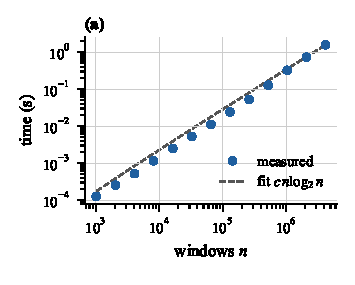
\includegraphics{greedy/figures/scaling}\hfill
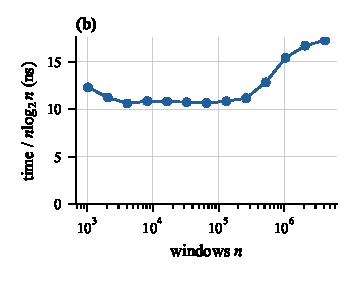
\includegraphics{greedy/figures/ratio}\hfill
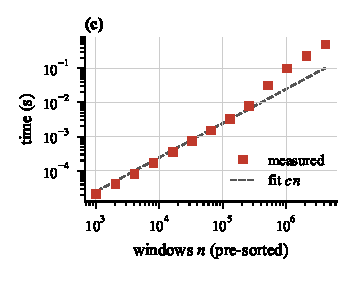
\includegraphics{greedy/figures/scan}
\caption{\textsc{Refresh-Days} on random windows. (a)~Running time with the
least-squares fit $c\,n\log_2 n$. (b)~Running time divided by
$n\log_2 n$; a flat curve confirms the growth rate. (c)~The scan alone on
pre-sorted windows, with the fit $c\,n$ over $n\le2^{17}$.}
\label{fig:greedy-scaling}
\end{figure*}

\begin{figure}[!t]
\centering
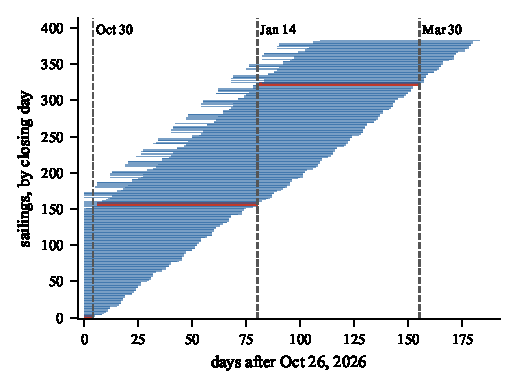
\includegraphics[width=\columnwidth]{greedy/figures/windows}
\caption{Quote windows of the $383$ real sailings, sorted by closing day.
Dashed lines are the three refresh days; the three witnesses are drawn
thick and red.}
\label{fig:greedy-windows}
\end{figure}

\textbf{Setup.} \textsc{Refresh-Days} was implemented in Python~3.12.2
(Appendix~\ref{app:greedy-code}) using the built-in sort, Timsort with the
powersort merge policy since Python~3.11~\cite{munro2018nearly}, and run on an AMD
Ryzen~7 9800X3D, following the protocol of Section~\ref{sec:dc-experiments}.
For $n=2^{10},\dots,2^{22}$ windows, departure days were drawn uniformly over
a horizon of $2n$ days, so that closing days are mostly distinct; a fixed
two-year horizon would make most windows tie. Cruise lengths were drawn from
the $383$ real sailings and windows built by~\eqref{eq:greedy-window} with
$c=2$. Each size was run five times on fresh inputs; we report the fastest
run with garbage collection disabled, as \texttt{timeit}
does~\cite{python-timeit}. Every run was checked to hit every window
(Lemma~\ref{lem:greedy-cover}) with one disjoint witness per day
(Lemma~\ref{lem:greedy-disjoint}). We also timed the scan alone on windows
already sorted by closing day. Unit tests additionally compare the output
with brute-force search on $300$ random instances of up to $10$ windows; this
checks the implementation on small cases, in the style of property-based
testing~\cite{claessen2000quickcheck}, and is not part of the proof.

\textbf{Running time.} Fig.~\ref{fig:greedy-scaling}(a) shows the time
following $c\,n\log_2 n$ over a $4096\times$ range of $n$, from
$0.1$\,ms to $1.6$\,s. In Fig.~\ref{fig:greedy-scaling}(b) the ratio is flat,
between $10.6$ and $12.3$\,ns, up to $n=2^{18}$, then rises to $17.3$\,ns at
$n=2^{22}$. The scan alone (Fig.~\ref{fig:greedy-scaling}(c)) costs
$20$ to $25$\,ns per window up to $n=2^{17}$, then up to $117$\,ns at
$n=2^{22}$. Both rises start around where the input, a list of Python tuples, no
longer fits in the processor's cache, and they are consistent with cache
misses~\cite{drepper2007memory}: after sorting, consecutive windows lie far apart in memory. Copying
the sorted windows into freshly allocated tuples cut the scan at $n=2^{22}$
from $118$ to $70$\,ns per window. The output size grew linearly, one refresh
day per about $39$ windows. Within the cache, the measurements match
Theorem~\ref{thm:greedy-time}: $n\log n$ with the sort, linear without it.


% Divide-and-conquer half of the report.
% Preamble needs: amsmath, amssymb, algorithmic, graphicx, cite, and
%   \newtheorem{lemma}{Lemma}  \newtheorem{theorem}{Theorem}
% \dcdir is the folder holding figures/ (empty when compiled from this folder).

\section{Divide and Conquer: Capped Map Search}
\label{sec:dc}

\subsection{Problem}
\label{sec:dc-problem}

Airbnb's map search returns the listings inside the visible map window, but
never more than a fixed number of them: a crowded window is silently
truncated. A market study of a city needs \emph{every} listing, so a scraper
must choose map windows small enough that none is truncated, using as few
searches as possible. This problem came up while scraping Miami, FL and
Rinc\'on, PR~\cite{danial2023airbnb}; a single city-wide window returned only a
small fraction of the listings.

\subsection{Abstraction}
\label{sec:dc-abstraction}

Let $P$ be a set of $n$ \emph{listings}, each with a location in
$\mathbb{R}^2$. Several listings may share a location, since Airbnb rounds
coordinates; let $m$ be the largest number sharing one. A \emph{window} is a
half-open rectangle $r=[x_0,x_1)\times[y_0,y_1)$, and $P_r$ denotes the
listings located in $r$. The search region $R$ is a window with $P_R=P$.

The search service is an oracle with cap $k\ge1$:
\begin{equation}
Q_k(r)=\begin{cases}
P_r & \text{if } |P_r|\le k,\\
\textsc{overflow} & \text{otherwise.}
\end{cases}
\label{eq:oracle}
\end{equation}
The problem is to compute $P$ from $R$ and $Q_k$ using as few oracle calls
(web requests) as possible.

Splitting a window at its midpoint, both horizontally and vertically, gives
four equal \emph{quadrants}. Splitting recursively yields a
\emph{quadtree}~\cite{finkel1974quad,samet1984quadtree} whose leaves are the
windows actually read.

\subsection{Algorithm}
\label{sec:dc-algorithm}

\textsc{Collect} (Fig.~\ref{fig:dc-alg}) queries a window. If it is not
truncated, its listings are the answer. Otherwise the window is divided into
four quadrants, each is solved recursively, and the answers are united. The
full answer is $\textsc{Collect}(R)$.

\begin{figure}[t]
\begin{algorithmic}[1]
\STATE \textbf{function} \textsc{Collect}$(r)$
\STATE $A\gets Q_k(r)$
\IF{$A\neq\textsc{overflow}$}
  \RETURN $A$ \COMMENT{window fits under the cap}
\ENDIF
\STATE $r_1,\dots,r_4\gets$ quadrants of $r$ \COMMENT{divide}
\RETURN $\bigcup_{i=1}^{4}\textsc{Collect}(r_i)$ \COMMENT{conquer, combine}
\end{algorithmic}
\caption{Enumerating the listings in window $r$ through a capped oracle $Q_k$.}
\label{fig:dc-alg}
\end{figure}

% Placed here in the source so LaTeX can set it at the top of the next page;
% a figure* is always deferred to the page after the one where it appears.
\begin{figure*}[!t]
\centering
\includegraphics[width=\textwidth]{\dcdir figures/scaling}
\caption{Scaling with $n$ at $k=50$, for uniform and clustered listings.
(a)~Running time with the least-squares fit $c\,n\log_2(n/k)$
($R^2=0.995$ uniform, $0.996$ clustered). (b)~Running time divided by
$n\log_2(n/k)$; a flat curve confirms the growth rate. (c)~Requests issued,
against the lower bound $n/k$.}
\label{fig:dc-scaling}
\end{figure*}

\subsection{Correctness}
\label{sec:dc-correctness}

\begin{lemma}\label{lem:partition}
The four quadrants of a window $r$ partition $r$.
\end{lemma}
\begin{IEEEproof}
Let $(x_m,y_m)$ be the midpoint of $r$. For $(x,y)\in r$, exactly one of
$x<x_m$ and $x\ge x_m$ holds, and exactly one of $y<y_m$ and $y\ge y_m$; the
pair picks exactly one quadrant. Each quadrant lies in $r$ since
$x_0\le x_m\le x_1$ and $y_0\le y_m\le y_1$.
\end{IEEEproof}

Half-open windows are what make this work: a listing on a split line falls in
exactly one quadrant, so it is neither lost nor counted twice.

Scale $R$ to the unit square and let $\delta\in(0,1]$ be the smallest
coordinate-wise distance, $\max(|\Delta x|,|\Delta y|)$, between two listings at
different locations ($\delta=1$ if there is only one location).

\begin{lemma}\label{lem:height}
If $m\le k$, the recursion tree of $\textsc{Collect}(R)$ has height at most
$\lceil\log_2(1/\delta)\rceil$; in particular the algorithm terminates.
\end{lemma}
\begin{IEEEproof}
A window at depth $d$ has side $2^{-d}$, so two listings inside it at different
locations are less than $2^{-d}$ apart, i.e.\ $\delta<2^{-d}$. A window is split
only if it holds more than $k\ge m$ listings, hence listings at two or more
locations, hence $d<\log_2(1/\delta)$. So every split window has depth at most
$\lceil\log_2(1/\delta)\rceil-1$ and every window depth at most
$\lceil\log_2(1/\delta)\rceil$. A tree of bounded height with four children per
internal node is finite.
\end{IEEEproof}

\begin{theorem}\label{thm:correct}
If $m\le k$, $\textsc{Collect}(r)=P_r$ for every window $r$, and the leaf
windows partition $r$ with at most $k$ listings each.
\end{theorem}
\begin{IEEEproof}
Strong induction on the height $h$ of the recursion tree at $r$ (finite by
Lemma~\ref{lem:height}). If $h=0$, the oracle did not overflow, so
$|P_r|\le k$ and line~4 returns $Q_k(r)=P_r$; the only leaf is $r$. If $h>0$,
the algorithm recurses on the quadrants $r_1,\dots,r_4$, whose subtrees are
shorter than $h$, so by induction $\textsc{Collect}(r_i)=P_{r_i}$ and the leaves
under $r_i$ partition $r_i$ with at most $k$ listings each. By
Lemma~\ref{lem:partition} each listing of $P_r$ lies in exactly one $r_i$, so
$\bigcup_i P_{r_i}=P_r$ and the leaves of the four subtrees partition $r$.
\end{IEEEproof}

The condition $m\le k$ is also necessary: if more than $k$ listings share a
location, every window containing it overflows, so no strategy using $Q_k$
can reveal them.

Lemmas~\ref{lem:partition}--\ref{lem:height} and Theorem~\ref{thm:correct}
are also machine-checked in Lean~4~\cite{lean4} (Appendix~\ref{app:dc-lean}).
Reported coordinates have finite precision (Airbnb gives five decimals), so
the formalization works on an integer grid, where $\delta$ is one grid unit.
There Lemma~\ref{lem:height} reads: if $m\le k$, recursion depth
$\lceil\log_2 W\rceil$ suffices for a window of side $W$; combined with
Theorem~\ref{thm:correct} this gives total correctness. The real-valued form
of Lemma~\ref{lem:height} is proved only on paper. The nearest existing
formalizations, region quadtrees in Isabelle~\cite{nipkow2024quad,nipkow2024afp}
and $k$-d trees in Isabelle and Coq~\cite{rau2019kdtree,hamid2023kdtree},
obtain termination from a fixed grid exponent or from the point count
shrinking at each median split; neither covers a space-splitting tree over
arbitrary points, so the proof here was written from scratch.

\subsection{Running Time}
\label{sec:dc-analysis}

Let $N$ be the number of oracle calls and $T$ the total work when a node with
$|P_r|$ listings spends $\Theta(|P_r|+1)$ time returning or distributing them.
Let $h$ be the tree height.

Windows at one depth are disjoint (Lemma~\ref{lem:partition}), so each level
holds at most $n$ listings and at most $\lfloor n/(k+1)\rfloor$ split windows,
each holding at least $k+1$ listings. Internal nodes sit at depths
$0,\dots,h-1$ and have four children each, so
\begin{equation}
\lceil n/k\rceil\le N\le 1+4h\Big\lfloor\frac{n}{k+1}\Big\rfloor,
\qquad T=O\big(n(h+1)\big).
\label{eq:general}
\end{equation}
The lower bound holds because the leaves cover $P$ with at most $k$ listings
each. By Lemma~\ref{lem:height}, $T=O(n\log(1/\delta))$: the cost is governed
by how tightly listings crowd, not by $n$ alone.

In the balanced case, where each split sends about $n/4$ listings to each
quadrant (true in expectation for uniformly random locations),
\begin{equation}
T(n)=4\,T(n/4)+\Theta(n)\quad(n>k),
\label{eq:recurrence}
\end{equation}
with $T(n)=\Theta(1)$ for $n\le k$. With $a=b=4$ and
$f(n)=\Theta(n)=\Theta(n^{\log_b a})$, case~2 of the Master
Theorem~\cite{cormen2022introduction} gives $T(n)=\Theta(n\log n)$. Unrolling
the recursion shows the dependence on $k$: the tree is complete with
$L=\lceil\log_4(n/k)\rceil$ levels below the root, each costing $\Theta(n)$, so
\begin{align}
T(n)&=\Theta\!\left(n\log\frac{n}{k}\right),\label{eq:balanced}\\
N&=\sum_{i=0}^{L}4^i=\frac{4^{L+1}-1}{3}=\Theta\!\left(\frac{n}{k}\right),
\label{eq:requests}
\end{align}
within a constant factor of the $n/k$ requests any strategy must make.

\subsection{In the Language of the Problem}
\label{sec:dc-domain}

Search the whole city in one window. If the results fit on the pages the site
shows, record them. Otherwise cut the window into four equal tiles and repeat
on each. A listing exactly on a cut goes to the tile right of or above it, so
it is recorded once. Dense neighborhoods get zoomed into repeatedly; open water
is dismissed after one search. The number of searches is proportional to
$n/k$, the number of listings divided by the number shown per search, by
\eqref{eq:requests}. The only obstacle is an address with more listings than
the cap, such as an apartment building whose units share rounded coordinates:
no zoom level separates them, which is why Theorem~\ref{thm:correct} needs
$m\le k$. In Rinc\'on at most $7$ listings share a location, so any $k\ge7$
works.

\subsection{Experiments}
\label{sec:dc-experiments}

\begin{figure}[!t]
\centering
\includegraphics[width=\columnwidth]{\dcdir figures/depth_vs_delta}
\caption{Effect of packing $k+1$ listings into a square of side $\delta$
($n=10{,}000$, $k=50$): (a)~tree height, (b)~requests.}
\label{fig:dc-depth}
\end{figure}

\begin{figure}[!t]
\centering
\includegraphics[width=2.45in]{\dcdir figures/rincon_quadtree}
\caption{Windows chosen for 261 listings in Rinc\'on, PR ($k=20$).}
\label{fig:dc-rincon}
\end{figure}

\textbf{Setup.} \textsc{Collect} was implemented in Python~3.14
(Appendix~\ref{app:dc-code}) and run on an AMD Ryzen~7 9800X3D. The oracle is
simulated: each node partitions the listings it holds among its quadrants,
which is the $\Theta(|P_r|)$ step of \eqref{eq:recurrence}. We used $k=50$
and $n=2^{10},\dots,2^{19}$ listings in the unit square, either uniform or
drawn from $20$ Gaussian clusters ($\sigma=0.02$). Each size was run five
times on fresh random inputs; we report the fastest run with garbage
collection disabled, as \texttt{timeit} does~\cite{python-timeit}. Every run
was checked to return each listing exactly once.

\textbf{Running time.} Fig.~\ref{fig:dc-scaling}(a) shows measured time
against the fitted model; Fig.~\ref{fig:dc-scaling}(b) divides time by
$n\log_2(n/k)$. Over a $512\times$ range of $n$ the ratio stays within
$26$--$43$\,ns (uniform) and $36$--$48$\,ns (clustered), confirming
$\Theta(n\log(n/k))$. The zig-zag arises because the tree gains a level only
when $n$ grows about fourfold, so the true cost rises in steps; the slight rise
at the largest sizes is consistent with cache effects. Clustered inputs cost
about $20\%$ more because their trees are two levels taller.

\textbf{Requests.} Table~\ref{tab:dc-requests} compares requests on uniform
inputs with the exact balanced count \eqref{eq:requests}; they agree within
$3.1\%$. Fig.~\ref{fig:dc-scaling}(c) shows the count growing linearly,
parallel to the lower bound $n/k$.

\begin{table}[t]
\caption{Requests on uniform inputs ($k=50$) vs.\ the prediction \eqref{eq:requests}}
\label{tab:dc-requests}
\centering
\begin{tabular}{rrrr}
\hline
$n$ & measured & predicted & height \\
\hline
1{,}024   & 85     & 85     & 3 \\
4{,}096   & 333    & 341    & 4 \\
16{,}384  & 1{,}337  & 1{,}365  & 5 \\
65{,}536  & 5{,}293  & 5{,}461  & 6 \\
262{,}144 & 21{,}197 & 21{,}845 & 7 \\
524{,}288 & 21{,}917 & 21{,}845 & 8 \\
\hline
\end{tabular}
\end{table}

\textbf{Crowding.} To test \eqref{eq:general}, we fixed $n=10{,}000$ uniform
listings and added $k+1=51$ listings inside a square of side
$\delta=2^{-2},\dots,2^{-28}$. Fig.~\ref{fig:dc-depth} shows the tree height
tracking $\log_2(1/\delta)$ (Lemma~\ref{lem:height}) although $n$ is fixed,
and each extra level adding about four requests, the $4h$ term of
\eqref{eq:general}.

\textbf{Real data.} Fig.~\ref{fig:dc-rincon} runs the algorithm with $k=20$ on
$261$ Airbnb listings from Rinc\'on, PR (scraped March 29, 2023~\cite{danial2023airbnb}).
It used $57$ requests, $43$ windows and height $5$, within the bounds
$14\le N\le 241$ of \eqref{eq:general}. The two dense clusters are split
repeatedly; the outskirts are covered by a few large windows.


\section{Conclusion}

For the cruise-fare tracker, scanning quote windows by closing day and
refreshing on the last day of each window not yet served gives the fewest
refresh batches, and the windows that forced a refresh prove that no schedule
can do better. The algorithm is a sort followed by a linear scan; measured
times follow $n\log n$ until the largest inputs, where the cost per window
rises, consistent with cache misses. The
result rests on the modeling choices stated in Section~\ref{sec:greedy}:
equal-cost batches, one observation per window, and windows defined by the
final-payment deadline and an assumed booking cutoff. It minimizes calls to
the API, not missed fare changes.

For the capped map search, splitting overflowing windows into quadrants
collects every listing with a number of requests within a constant factor of
the $n/k$ lower bound when listings are spread evenly, and never recurses
deeper than $\lceil\log_2 W\rceil$ levels on a map of $W$ grid units. The
one assumption, that no single location holds more than $k$ listings, is
necessary for any strategy that only sees capped search results. Measured
running times follow the $\Theta(n\log(n/k))$ analysis over three orders of
magnitude, request counts match the balanced-case prediction within $3.1\%$,
and the correctness argument is machine-checked.

\bibliographystyle{IEEEtran}
\bibliography{refs}

% Code reads better at full page width.
\onecolumn
\appendices
% Appendices for the divide-and-conquer half. Needs \usepackage{listings}.

\section{Divide-and-Conquer Code}
\label{app:dc-code}

The algorithm (\texttt{quadtree.py}) and the measurements behind
Figs.~\ref{fig:dc-scaling}--\ref{fig:dc-depth} and Table~\ref{tab:dc-requests}
(\texttt{experiments.py}). The plotting script, the unit tests, the Rinc\'on
data file and the raw measurements are in the project
repository.\footnote{\url{https://github.com/IlanDanial/P1Alg}}

\lstinputlisting[language=Python,caption={quadtree.py}]{\dcdir quadtree.py}
\lstinputlisting[language=Python,caption={experiments.py}]{\dcdir experiments.py}

\section{Machine-Checked Proof}
\label{app:dc-lean}

Lemma~\ref{lem:partition} (\texttt{quadrants\_cover},
\texttt{quadrants\_disjoint}), Theorem~\ref{thm:correct}
(\texttt{collect\_correct}), Lemma~\ref{lem:height} on the integer grid
(\texttt{collect\_terminates}) and their combination into total correctness
(\texttt{collect\_total}) in Lean~4.35, using only the core library.
\texttt{lake build} in \texttt{divide\_and\_conquer/proof} checks it; the
theorems depend on no axioms beyond Lean's standard three
(\texttt{propext}, \texttt{Classical.choice}, \texttt{Quot.sound}).

\lstinputlisting[language={},caption={proof/Proof/Collect.lean}]{\dcdir proof/Proof/Collect.lean}

\section{LLM Usage: Divide-and-Conquer Part}
\label{app:dc-llm}

\textbf{Tool.} Claude Code (Anthropic's command-line coding agent), model
Claude Opus~5.5 (\texttt{claude-opus-5-5}), October 2026. The agent read the
assignment, read the scraper repository~\cite{danial2023airbnb}, searched the web
for the IEEE template, wrote and ran the code, and drafted this section. All
proofs, numbers, and citations were checked by the authors.

\textbf{Prompts (verbatim).}
\begin{enumerate}
\item ``DO you understand the project I need to do also this is a group project
  I am doing the divide an conquer part''
\item ``My Idea for the problem is a problem I have solved before with divide
  and conquer \url{https://github.com/IlanDanial/airbnb_data} I split the map over and
  over, each time checking the amount of properties in the split and if it was
  under I took those properties and added it to the list since you can only see
  so many properties at a time''
\item ``yes start the implementation, we're using IEEE search online for proper
  template''
\item ``yes write the LaTeX section''
\item ``This is really ugly'' followed by ``My bigger issue is that the
  explanations are very longwinded for no reason and the formatting of the
  page is ugly its hard to read as well''
\item ``I have an issue with some of this read the paper be critical how do
  you think of the formatting'', then ``fix all of them at once'' and ``also
  do we need the full code in the appendix or can we reference a repository''
\item ``would it be worth it to look at the code and refactor it and the
  comments in the code'', then ``go''
\item ``Isnt there a code languge that is built to prove proofs can we use
  that to prove correctness'', then ``I want to go for it also I am sure there
  are online proofs of this exact same thing in the same language so it should
  take less than an hour''
\item ``so your telling me that there was no problem with proving the whole
  thing end to end''
\item ``actually search online for the hard part dont just tell me it does
  not exist''
\item ``do both, go for the full proof, or is there a solution we can do that
  would be easier to prove and solve the problem all the same''
\end{enumerate}

\textbf{Results.}
% TODO: paste the full exported transcript (Claude Code: /export) here or in
% supplementary material; the assignment requires all intermediate results.
(1)~A summary of the assignment and four candidate divide-and-conquer problems.
(2)~An analysis of the scraper's \texttt{subdivide} recursion as an adaptive
quadtree, identifying the termination issue for co-located listings and the
double-counting issue on window borders.
(3)~\texttt{quadtree.py}, \texttt{test\_quadtree.py}, \texttt{experiments.py},
and the figures; an intermediate run stopped when the minimum-width guard was
reached, after which the crowding experiment was limited to
$\delta\ge2^{-28}$, and garbage collection was disabled during timing.
(4)~A first draft of Section~\ref{sec:dc} and these appendices, with five
separate figures in matplotlib's default style.
(5)~The draft was shortened by about a third, the five figures were
restyled to match the paper's typeface and merged into three, and the page
layout was fixed.
(6)~A list of nine formatting defects (an equation label pushed to its own
line, a wrapped pseudocode line, mixed paragraph styles, inconsistent
equation citations, a legend mismatch), all then fixed; the unit tests were
removed from this appendix in favor of the repository link.
(7)~The plotting code was split out of \texttt{experiments.py} into
\texttt{plots.py}, and docstrings and comments were added.
(8)~An assessment of proof assistants (Lean~4, Coq, Isabelle, Dafny) and of
which parts of the proof are feasible to formalize; then a first Lean
formalization of Lemma~\ref{lem:partition} and Theorem~\ref{thm:correct}
only, with \textsc{Collect} given a fuel bound, which compiled on the first
build.
(9)~A clarification that this was partial correctness, not an end-to-end
proof, with three further gaps listed (integer midpoints, the oracle not being
a black box, no duplicate-freeness proof).
(10)~A web search that found the Isabelle and Coq formalizations cited in
Section~\ref{sec:dc-correctness}, none covering separation-based termination;
the assistant's earlier claim that no related formalization existed was
withdrawn.
(11)~The observation that finite-precision coordinates make the problem a
grid problem, on which Lemma~\ref{lem:height} is provable by induction on the
depth; \texttt{collect\_terminates} and \texttt{collect\_total} were then
added, needing one round of fixes to core-library lemma names before
compiling.

% Appendices for the greedy half. Needs \usepackage{listings}.
% Paths are relative to the repository root, where report.tex lives.

\section{Greedy Code}
\label{app:greedy-code}

The algorithm (\texttt{refresh\_days.py}) and the measurements behind
Fig.~\ref{fig:greedy-scaling} (\texttt{experiments.py}). The unit tests
(\texttt{test\_refresh\_days.py}), the download script
(\texttt{fetch\_sailings.py}), the plotting script, the sailing data and the
raw measurements are in the \texttt{greedy/} folder of the project
repository.\footnote{\url{https://github.com/IlanDanial/P1Alg}}

\lstinputlisting[language=Python,caption={refresh\_days.py}]{greedy/refresh_days.py}
\lstinputlisting[language=Python,caption={experiments.py}]{greedy/experiments.py}

\section{Greedy Machine-Checked Proof}
\label{app:greedy-lean}

Lemma~\ref{lem:greedy-cover} (\texttt{refresh\_covers}),
Lemma~\ref{lem:greedy-disjoint} (\texttt{witnesses\_pairwise\_disjoint}) and
Theorem~\ref{thm:greedy-opt} (\texttt{refresh\_optimal}) in Lean~4.35, using
only the core library. \texttt{lake build} in \texttt{greedy/proof} checks
it; the theorems depend on no axioms beyond Lean's standard three
(\texttt{propext}, \texttt{Classical.choice}, \texttt{Quot.sound}).

\lstinputlisting[language={},caption={proof/Proof/Refresh.lean},
  literate={≤}{{$\le$}}1 {≠}{{$\ne$}}1 {∧}{{$\wedge$}}1 {∨}{{$\vee$}}1
           {¬}{{$\neg$}}1 {→}{{$\rightarrow$}}1 {∀}{{$\forall$}}1
           {∃}{{$\exists$}}1 {⟨}{{$\langle$}}1 {⟩}{{$\rangle$}}1
           {×}{{$\times$}}1 {∈}{{$\in$}}1 {·}{{$\cdot$}}1 {…}{{$\ldots$}}1
           {∞}{{$\infty$}}1]{greedy/proof/Proof/Refresh.lean}

\section{LLM Usage: Greedy Part}
\label{app:greedy-llm}

\textbf{Tools.} (1)~A GPT-6 Astra brainstorming session that utilized back and forth questioning to get a rough concept of a plan. (2)~A GPT-6 Astra thread that reviewed and revised the project prompt. (3)~This
implementation session: Claude Code (Anthropic's command-line coding agent),
model Claude Opus~5.5 (\texttt{claude-opus-5-5}), which wrote the code, reviewed
the experiments, and revised the draft report and Section~\ref{sec:greedy}.

\textbf{Prompt (verbatim).} The project implementation session was driven by the
single prompt below, reproduced exactly.

\lstinputlisting[language={},caption={Implementation prompt},
  literate={×}{{$\times$}}1 {…}{{$\ldots$}}1 {′}{{$'$}}1 {←}{{$\leftarrow$}}1
           {→}{{$\rightarrow$}}1 {∀}{{$\forall$}}1 {∅}{{$\emptyset$}}1
           {∈}{{$\in$}}1 {−}{{$-$}}1 {∞}{{$\infty$}}1 {≤}{{$\le$}}1
           {≥}{{$\ge$}}1]{greedy/appendix/prompt.md}

\textbf{Results, by step.}
(1)~\texttt{refresh\_days.py}: \texttt{refresh\_days} returns the days and
the witnesses; \texttt{windows} builds clipped windows from sailing dates; a
separate \texttt{refresh\_days\_sorted} holds the scan alone for the
pre-sorted experiment.
(2)~\texttt{test\_refresh\_days.py} with the five requested checks and a
check that a reversed interval raises \texttt{ValueError}. All six tests
passed on the first run.
(3)~\texttt{fetch\_sailings.py} downloaded six months of sailings on
October 26, 2026: one page per month (no month exceeded $200$ itineraries),
$383$ sailings, every duration equal to arrival minus departure. With
$c=2$: $n=383$ windows, $m=3$ refresh days (October 30, 2026; January 14,
2027; March 30, 2027), horizon $184$ days. Carnival's help page returned
HTTP~403 to scripted requests and never finished loading in a browser, so the
$76$- and $91$-day deadlines were read from the Internet Archive's copy of
the same page (July 23, 2025), cited in~\cite{carnival481}. That table counts
cruise length in days; the session checked that the ``$N$-Day'' itinerary
titles, the duration field, and arrival minus departure agree on all $383$
sailings, so the $5$-or-fewer rule applies to the duration field directly.
(4)~\texttt{experiments.py} and \texttt{plots.py}, about one minute to run.
The full algorithm fit $c\,n\log_2 n$ with $R^2=0.998$. The scan alone grew
from $20$ to $117$\,ns per window above $n=2^{17}$; a follow-up timing that
re-allocated the sorted tuples in memory order reduced this to $70$\,ns at
$n=2^{22}$, which supports, but does not prove, the cache explanation in
Section~\ref{sec:greedy-experiments}. After the first compile, the
least-squares line in Fig.~\ref{fig:greedy-scaling}(c) sat above every
in-cache point because the large sizes dominated it, so the fit was
restricted to $n\le2^{17}$ and the caption says so; legends that covered
data points were moved.
(5)~Section~\ref{sec:greedy}, the bibliography entries, and the front
matter, introduction and conclusion in \texttt{main.tex}.
(6)~Tectonic is not in the \texttt{winget} catalog (both the package id and
a search returned nothing), so MiKTeX was installed with \texttt{winget},
with on-the-fly package installation enabled.
(7)~This appendix, \texttt{greedy/README.md} and the top-level
\texttt{README.md}.
(8)~Verification: unit tests, presence of every output file, and
\texttt{git status} listing only the permitted paths.
(9)~Lean formalization. The official \texttt{elan} installer was run (its
first invocation failed on a PowerShell argument-type error and was rerun);
\texttt{lake build} of the divide-and-conquer proof succeeded, installing
Lean~4.35.0. \texttt{greedy/proof/Proof/Refresh.lean} defines the scan with
$\mathit{last}$ as an \texttt{Option Int} argument (\texttt{none} for
$-\infty$) returning the witnesses, and proves \texttt{refresh\_covers},
\texttt{witnesses\_pairwise\_disjoint} and \texttt{refresh\_optimal}.

\textbf{Full transcripts.} The prompts, tool calls and responses of every
session, in order, are in the repository at
\texttt{greedy/appendix/transcript.md}. To the best of my knowledge they
comply with the LLM policies of the course.


\end{document}
